\section{Обучение с подкреплением} \label{ch1:rl}

Хотя алгоритмы \hyperref[acr:rl]{RL} эффективно решают различные задачи, им не хватает масштабируемости и размерности.

С ростом глубоких нейронных сетей в последние годы, RL начинает использовать их функции приближения и представления свойств \cite{HORNIK1991251}. Это помогает преодолеть недостатки алгоритмов RL.

Это устраняет необходимость описывать свойства вручную, позволяя обучать модели, способные непосредственно выводить оптимальные действия, на основе необработанного и высокоразмерного ввода с сенсоров. Это проиллюстрировано на \firef{fig:DRL-flow}.

Таким образом, использование ИНС в обучении подкреплением, создает новую область – глубокое обучение с подкреплением (Deep Reinforcement Learning, DRL).


\subsection{Алгоритмы глубокого обучения с подкреплением}

Здесь нужно рассказать о \hyperref[acr:mdp]{Марковском процессе принятия решений} (Markov Decision Process, MDP).

\subsubsection{Марковский процесс принятия решений}

Свойство Маркова означает, что следующее состояние зависит только от текущего состояния, тем самым, при принятии решения, мы можем игнорировать все прошлые состояния и учитывать только текущее.

Процесс {\itshape обучения с подкреплением} является формой \hyperref[acr:mdp]{МППР}. Он состоит из нескольких элементов:

\begin{itemize}
	\item набор состояний окружающей среды $S$;
	\item набор действий $A$;
	\item динамика перехода $T(s_{(t+1)}|s_t, a_t)$, которая описывает распределение новых состояний $s_{t+1}$, в которые может попасть агент, совершив действие $a_t$ в состоянии $s_t$;
	\item функция награды $R(s_t; a_t; s_{t+1})$
	\item дискаунт фактор $\gamma \in [0, 1]$ для экспоненциального снижения будущих наград.
\end{itemize}

Политика $\pi$ сопоставляет состояния вероятностям распределения действий: $\pi : S \to p(A = a|S)$

Эпизод --- это предопределенный период времени, когда среда, начиная со случайного состояния, порождает серию переходов. Переходы в эпизоде можно рассматривать как траекторию политики.

Сумма наград, собранных в траектории политики $R = \sum_{t=0}^{T-1} \gamma^t r_{t+1}$

Цель обучения с подкреплением состоит в том, чтобы изучить оптимальную политику ${\pi^*}$, которая максимизирует ожидаемую награду из всех состояний, $\pi^* = argmax_x \mathbb{E} [R|\pi]$ \cite{Otterlo2012ReinforcementLA}

\subsection{Подход, основанный на функции состояния (Value Based подход)}

Этот подход состоит в том, чтобы оптимизировать значение функции $V(s)$.

value-функция — это функция, которая сообщает нам максимальное ожидаемое будущее вознаграждение, которое агент получит в каждом состоянии. Значение каждого состояния — это общая сумма вознаграждений, на которую агент может рассчитывать в будущем, начиная с этого состояния.

\begin{equation} \label{eq:someEq}
V^\pi (s) = \mathbb{E}^\pi [R_{t+1} + \gamma R{t+2} + \gamma^2 R{t+3} + ... |S_t = s]
\end{equation}
% TODO: \pi сверху или снизу

\paragraph{Q-обучение}

Функция состояния-значения (state-value funcrion) $V^\pi (s) = \mathbb{E}[R|s, \pi]$ --- ожидаемая награда с данными состоянием $s$ и политикой $\pi$. В то же время, в RL такой переход $T$ не всегда возможен, поэтому, обычно используется другая функция состояния-значения или функция качества $Q^\pi(s,a) = \mathbb{E}[R|s, a, \pi]$. Оптимальная политика получается через выбор на каждом шаге действия, которое максимизирует Q-функцию \cite{SuttonAndBarto-RL-Introduction-p107}. Q-обучение -- это алгоритм без политики (off-policy), так как он жадно выбирает действие исходя из текущего состояния, вместо того, чтобы следовать политике.

Для рекурсивного изучения $Q^\pi$, применяется {\itshape уравнение Беллмана}:

\begin{equation} \label{eq:q-learning-bellmanEq}
Q^\pi(s_t, a_t) = \mathbb{E}_{s_{t+1}}[r_{t+1} + \gamma Q^\pi (s_{t+1}, \pi(s_{t+1}))]
\end{equation}

Традиционное Q-обучение способно сформулировать оптимальную политику обучением состояние-действие-значение функции. Однако, оно предназначено для дискретных пространств действий с малым количеством измерений и не способно решать более-менее сложные задачи.

\paragraph{Глубокая Q-сеть (DQN)}

Глубокая Q-сеть (DQN) --- вариант Q-обучения, который использует глубокую сверточную нейронную сеть для вычисления Q-функции. Является прорывом в обучении с подкреплением. \cite{bertsekas1996neuro}

DQN была применена в игре Atari и достигла производительности, сопоставимой с человеческим уровнем. \cite{Mnih2015}

Для решения проблемы нестабильности и расхождения нелинейных функций аппроксиматоров, таких как нейронные сети, был применен метод {\itshape Experience Replay} [17]. Идея Experience Replay в том, чтобы равномерно рандомизировать предыдущие переходы при обучении модели, которое нарушает корреляцию последовательности наблюдений. Опыт агента $e_t = (s_t, a_t, r_t, s_{t+1)}$ на каждом шаге $t$ сохраняется в буфер $D_t = {e_1, ..., e_t}$. Во время тренировки модели случайным образом извлекается небольшая часть опыта $(s; a; r; s') ~ U(D)$.

\paragraph{Двойная глубокая Q-сеть (Double DQN, DDQN)}

Это ещё один вариант DQN, в котором используется две Q-сети.

Текущая Q-сеть $Q(s, a; \theta_i)$ обновляется итеративно во время обучения, а целевая Q-сеть $Q(s', a'; \theta_i^\_)$ используется для получения целевого Q-значения и обновляется только периодически. Целевая Q-сеть уменьшает смещение, вызванное неточностями Q-сети в начале обучения.

На каждой итерации $i$ Q-сеть обновляется на ошибку темпоральной разницы (temporal difference, TD):

\begin{equation} \label{eq:someEq}
L_i(\theta_i) = \mathbb{E}^\pi [R_{t+1} + \gamma R{t+2} + \gamma^2 R{t+3} + ... |S_t = s]
\end{equation}

%Где $\gamma$ — это скорость затухания для будущих наград. ${\theta_i^{_}}$ параметры целевой Q-сети, и $\theta_i$ -текущей Q-сети на итерации.

DQN подошел к проблеме низкоразмерных входных данных наблюдения с применением глубоких нейронных сетей для извлечения свойств из высокомерного необработанного сенсорного сигнала, такого как пиксели изображения в играх. Тем не менее, он все еще ограничен его дискретным и низкоразмерным пространством действия.

\subsection{Линия поведения (Policy Based)}

Вместо получения оптимальной политики путем поддержания Q-функции, алгоритм напрямую ищет оптимальную политику путем максимизации ожидаемого значения $\mathbb{E}[R|\pi_\theta]$. Мы хотим итеративно подгонять параметр $\theta$ сети, так чтобы максимизировать $\mathbb{E}[R|\pi_\theta]$.

Оптимизация, основанная на градиенте, используется чаще, так как это более эффективно, при работе с большими сетями со множеством параметров. \cite{Arulkumaran_2017}

\subsubsection{Policy Gradients} (TODO: перевод?)

Нейронная сеть, которая представляет параметризованную политику обновляется при изучении сигналов в методах Policy Gradients. В RL без модели, для оценки градиента на примерах, сгенерированных в траектории политикой, используется правило {\itshape REINFORCE} или функция оценки. Предположим, что f(х) – это функция оценки, где $x$ - случайная величина для одного перехода. Градиент политики может быть рассчитан с использованием отношения правдоподобия:

\begin{equation}
	\label{eq:ch1-likelihood-ratios}
	\begin{multlined}
		\nabla_\theta \mathbb{E}_x[f(x)] = \mathbb{E}_x[f(x) \nabla_\theta \log p x|\theta]
	\end{multlined}
\end{equation}

Теперь рассмотрим траекторию $\tau$ с переходами $(a_t, s_t, r_t, s_t+1)$ в соответствии с политикой, тогда градиент политики это:

\begin{equation}
\label{eq:ch1-likelihood-ratios}
\begin{multlined}
\nabla_\theta \mathbb{E}[R_\tau] = \mathbb{E}[\sum_\tau R_\tau \nabla_\theta \log \pi {a_\tau|s_\tau;\theta}]
\end{multlined}
\end{equation}

Недостатком policy gradient является низкая скорость работы — требуется большое количество вычислений для подсчета награды. Так же policy gradient может застрять в локальном оптимуме, не найдя глобального.

\subsubsection{Актор-критик}

Так как value-функция может предоставить обучающие сигналы для прямого оптимального поиска политики, естественным было объединить два подхода.

В DRL две нейронные сети, представляющие актора и критика соответственно, используются для приближения функции, где актор (политика) учится по Q-значениям, оцененным критиком (value-функция) \cite{Arulkumaran_2017}. \firef{fig:ch1-RL-actor-critic} показывает, как актор и критик сети взаимодействуют с окружающей средой.

\begin{figure}[ht!]
	\center
	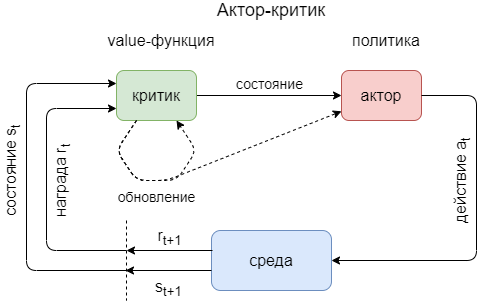
\includegraphics [scale=0.60] {my_folder/images/ch1/RL-actor-critic.png}
	\caption{{\itshape Актор} получает состояние из окружающей среды и реагирует на действие, {\itshape критик} получает состояние и награду и рассчитывает TD ошибку для обновления себя и {\itshape актора}. Основано на \cite{Arulkumaran_2017}}
	\label{fig:ch1-RL-actor-critic}
\end{figure}

\subsubsection{Глубокий детерминированный градиент политики (DDPG)}

\hyperref[acr:ddpg]{DDPG} - актор-критик алгоритм без модели и без политики \cite{lillicrap2015continuous}. Он расширяет \hyperref[acr:dpg]{DPG} использованием глубоких нейронных сетей. Так же, он использует хорошо зарекомендовавший себя приём DQN с текущей и целевой Q-сетями (сети критиков) и experience replay, чтобы стабилизировать обучение. И, наконец, он использует детерминистическую политику (сеть акторов) вместо политики стохастического поведения.
В отличие от стохастической политики, которая определяет вероятность распределения через действия, в данном состоянии, детерминированность в DDPG подразумевает, что конкретное действие аппроксимируется в данном состоянии. Соответственно, конкретное состояние для следующего шага, так же детерминировано.
Следовательно, вместо использования рекурсивного программирования, как в уравнении {\itshape Беллмана}, используется детерминированная политика $\mu : S \leftarrow A$ \cite{lillicrap2015continuous}

\begin{equation}
	\label{eq:ch1-ddpg-1}
	\begin{multlined}
		Q^\mu (s_t, a_t) = \mathbb{E}_{r_t, s_{t+1}~E}[r(s_t, a_t) + \gamma Q^\mu(s_{t+1}, \mu(s_{t+1})]
	\end{multlined}
\end{equation}

что очень похоже на Q-обучение – алгоритм с жадной политикой. Сеть критика обновляется по функции потерь:

\begin{equation}
	\label{eq:ch1-ddpg-1}
	\begin{multlined}
		L(\theta^Q) = \mathbb{E}[(Q(s_t, a_t|\theta^Q) - y_t)^2]
	\end{multlined}
\end{equation}

где

\begin{equation}
	\label{eq:ch1-ddpg-3}
	\begin{multlined}
		y_t = r(s_t, a_t) + \gamma Q(s_{t+1}, \mu(s_{t+1})j\theta^Q)
	\end{multlined}
\end{equation}

Сеть актора обновляется функцией потерь:

\begin{equation}
	\label{eq:ch1-ddpg-4}
	\begin{multlined}
		\nabla_{\theta \mu} J \approx \mathbb{E}[\nabla_{\theta \mu} Q(s, a \theta^Q)|_{s=s_t,a=\mu(s_t|\theta^\mu)}] \\
		= \mathbb{E}[\nabla_a Q(s, a \theta^Q)|_{s=s_t,a=\mu(s_t) \nabla_{\theta \mu} \mu (s|\theta^\mu)|s=s_t}]
	\end{multlined}
\end{equation}

Как и в DQN, чтобы избежать расхождения, DDPG применяет мягкое обновление для целевых сетей критика и актора. Они обновляются только раз в указанное количество шагов.
